% DOC SETTINGS ===================================
\documentclass{article}
\usepackage[utf8]{inputenc}
\usepackage{fancyhdr}
\pagestyle{fancy}
\usepackage{geometry}
 \geometry{
 a4paper,
 total={170mm,257mm},
 left=20mm,
 top=25mm,
 }
\fancyheadoffset{0mm}
\lhead{ECE3544 Lab 1.B Report}
\rhead{Kavin Thirukonda 2021}
\usepackage{steinmetz}
\usepackage{listings}
\usepackage{longtable}
\usepackage{circuitikz}
\usepackage{mathtools}  
\mathtoolsset{showonlyrefs} 
\cfoot{}
% DOC SETTINGS ===================================
\begin{document}
\begin{center}
    \vspace*{1cm}
    \Huge
    \textbf{ECE3544 Lab 1 Report}
    
    \vspace{0.5cm}
    \LARGE
    Section B
    
    \vspace{1.5cm}
    \textbf{Kavin Thirukonda}
    \vfill
    \small
    Description:
    
    This is the formal lab report for Lab 1.B to discuss the objectives, constraints, design, optimization, and implementation of Lab 1.B.
    \vspace{10cm}
\end{center}
\newpage
\section{Objectives}
The objectives of this project is to become more familiar with verilog continuous code once again as well as modelsim coding and testing. That includes using the model sim program itself as well as launching waveform test benches, also making project, coding .v files, and making test benches.
\section{Planning}
\subsection{Test Bench Comparisons}
The key difference between the two test bench files as far as I see is the choice to use a for loop to cut down the repetition in the code, since most of the lines in the first file were very similar bar one or two bits changing.

While both of these methods are effective at completing the task, when creating large test benches for bigger projects it would surely benefit you to use the for loops to test repetitive functions.
\subsection{Simulation Results}
\begin{center}
    \boxed{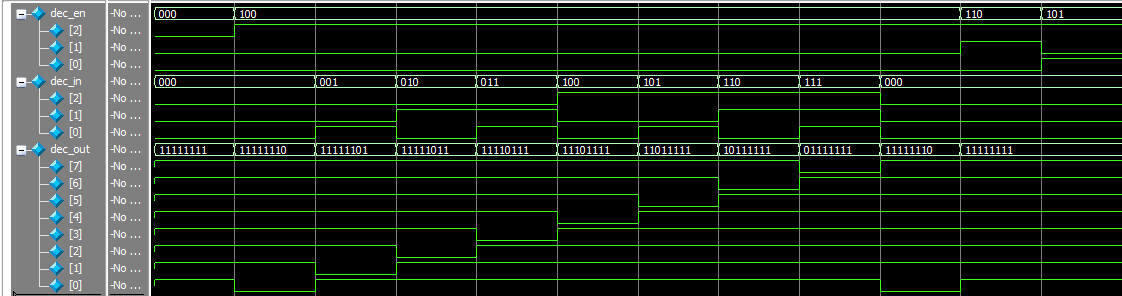
\includegraphics[width = .95\textwidth]{38decoder.png}}
    
    Above are the simulation results of the 3 to 8 decoder
\end{center}

\begin{center}
    \boxed{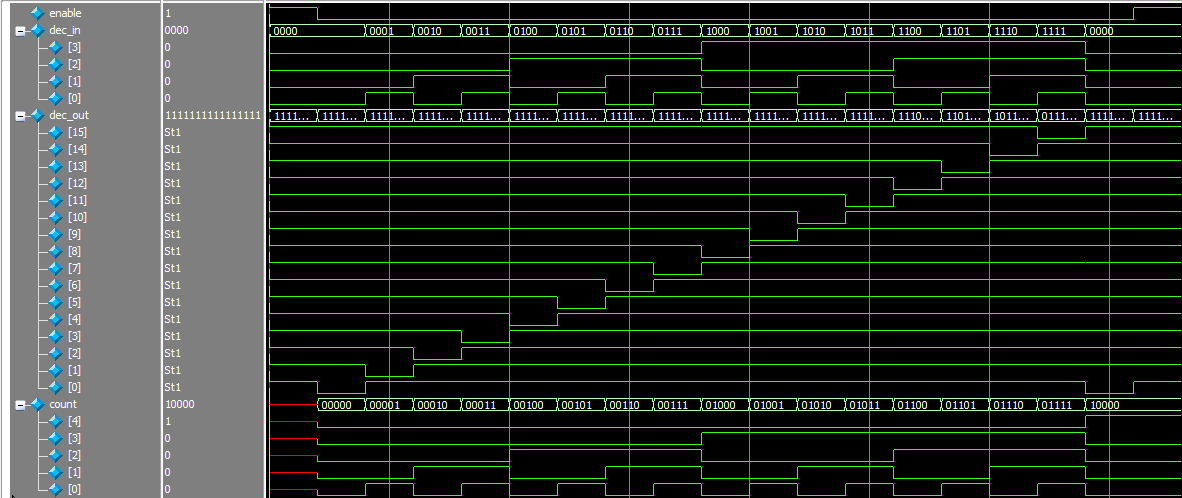
\includegraphics[width = .95\textwidth]{416decoder.png}}
    
    above are the simulation results of the 4 to 16 decoder
\end{center}
\section{Implementation}
\subsection{RPS Design Approach}
The design approach I chose this time was to use some basic all nand circuits to determine if the game was tied, or one of the players won. And from there if none of those were true the game was set to rematch because that was the most complicated logic to implement and only one output can be true at once so having that logic works.

Compared to the design approach I chose last time this was not as transistor efficient but it was much more time efficient and if there was a problem it could more easily be debugged. This is a design approach that can be scaled because Instead of shoving it all into several kmaps (like I did in project 1A) I used the problem specification to help me find a simpler solution.
\newpage

\subsection{RPS Truth Table}

\begin{center}
    \renewcommand{\arraystretch}{.95}
    \begin{tabular}{c|c|c|c|c|c|c|c|c|c|c}
        a[1] & a[0] & b[1] & b[0] & c[1] & c[0] & P1 & P2 &  P3 & TIE & REMATCH \\
        \hline
        0  &  0  &  0  &  0  &  0  &  0  &  0  &  0  &  0  &  1  &  0 \\
        0  &  0  &  0  &  0  &  0  &  1  &  X  &  X  &  X  &  X  &  X \\
        0  &  0  &  0  &  0  &  1  &  0  &  0  &  0  &  0  &  0  &  1 \\
        0  &  0  &  0  &  0  &  1  &  1  &  0  &  0  &  1  &  0  &  0 \\
        0  &  0  &  0  &  1  &  0  &  0  &  X  &  X  &  X  &  X  &  X \\
        0  &  0  &  0  &  1  &  0  &  1  &  X  &  X  &  X  &  X  &  X \\
        0  &  0  &  0  &  1  &  1  &  0  &  X  &  X  &  X  &  X  &  X \\
        0  &  0  &  0  &  1  &  1  &  1  &  X  &  X  &  X  &  X  &  X \\
        0  &  0  &  1  &  0  &  0  &  0  &  0  &  0  &  0  &  0  &  1 \\
        0  &  0  &  1  &  0  &  0  &  1  &  X  &  X  &  X  &  X  &  X \\
        0  &  0  &  1  &  0  &  1  &  0  &  0  &  0  &  0  &  0  &  1 \\
        0  &  0  &  1  &  0  &  1  &  1  &  0  &  0  &  0  &  0  &  1 \\
        0  &  0  &  1  &  1  &  0  &  0  &  0  &  1  &  0  &  0  &  0 \\
        0  &  0  &  1  &  1  &  0  &  1  &  X  &  X  &  X  &  X  &  X \\
        0  &  0  &  1  &  1  &  1  &  0  &  0  &  0  &  0  &  0  &  1 \\
        0  &  0  &  1  &  1  &  1  &  1  &  1  &  0  &  0  &  0  &  0 \\
        0  &  1  &  0  &  0  &  0  &  0  &  X  &  X  &  X  &  X  &  X \\
        0  &  1  &  0  &  0  &  0  &  1  &  X  &  X  &  X  &  X  &  X \\
        0  &  1  &  0  &  0  &  1  &  0  &  X  &  X  &  X  &  X  &  X \\
        0  &  1  &  0  &  0  &  1  &  1  &  X  &  X  &  X  &  X  &  X \\
        0  &  1  &  0  &  1  &  0  &  0  &  X  &  X  &  X  &  X  &  X \\
        0  &  1  &  0  &  1  &  0  &  1  &  X  &  X  &  X  &  X  &  X \\
        0  &  1  &  0  &  1  &  1  &  0  &  X  &  X  &  X  &  X  &  X \\
        0  &  1  &  0  &  1  &  1  &  1  &  X  &  X  &  X  &  X  &  X \\
        0  &  1  &  1  &  0  &  0  &  0  &  X  &  X  &  X  &  X  &  X \\
        0  &  1  &  1  &  0  &  0  &  1  &  X  &  X  &  X  &  X  &  X \\
        0  &  1  &  1  &  0  &  1  &  0  &  X  &  X  &  X  &  X  &  X \\
        0  &  1  &  1  &  0  &  1  &  1  &  X  &  X  &  X  &  X  &  X \\
        0  &  1  &  1  &  1  &  0  &  0  &  X  &  X  &  X  &  X  &  X \\
        0  &  1  &  1  &  1  &  0  &  1  &  X  &  X  &  X  &  X  &  X \\
        0  &  1  &  1  &  1  &  1  &  0  &  X  &  X  &  X  &  X  &  X \\
        0  &  1  &  1  &  1  &  1  &  1  &  X  &  X  &  X  &  X  &  X \\
        1  &  0  &  0  &  0  &  0  &  0  &  1  &  0  &  0  &  0  &  0 \\
        1  &  0  &  0  &  0  &  0  &  1  &  X  &  X  &  X  &  X  &  X \\
        1  &  0  &  0  &  0  &  1  &  0  &  0  &  1  &  0  &  0  &  0 \\
        1  &  0  &  0  &  0  &  1  &  1  &  0  &  0  &  0  &  0  &  1 \\
        1  &  0  &  0  &  1  &  0  &  0  &  X  &  X  &  X  &  X  &  X \\
        1  &  0  &  0  &  1  &  0  &  1  &  X  &  X  &  X  &  X  &  X \\
        1  &  0  &  0  &  1  &  1  &  0  &  X  &  X  &  X  &  X  &  X \\
        1  &  0  &  0  &  1  &  1  &  1  &  X  &  X  &  X  &  X  &  X \\
        1  &  0  &  1  &  0  &  0  &  0  &  0  &  0  &  1  &  0  &  0 \\
        1  &  0  &  1  &  0  &  0  &  1  &  X  &  X  &  X  &  X  &  X \\
        1  &  0  &  1  &  0  &  1  &  0  &  0  &  0  &  0  &  1  &  0 \\
        1  &  0  &  1  &  0  &  1  &  1  &  0  &  0  &  0  &  0  &  1 \\
        1  &  0  &  1  &  1  &  0  &  0  &  0  &  0  &  0  &  0  &  1 \\
        1  &  0  &  1  &  1  &  0  &  1  &  X  &  X  &  X  &  X  &  X \\
        1  &  0  &  1  &  1  &  1  &  0  &  0  &  0  &  0  &  0  &  1 \\
        1  &  0  &  1  &  1  &  1  &  1  &  0  &  0  &  0  &  0  &  1 \\
        1  &  1  &  0  &  0  &  0  &  0  &  0  &  0  &  0  &  0  &  1 \\
        1  &  1  &  0  &  0  &  0  &  1  &  X  &  X  &  X  &  X  &  X \\
        1  &  1  &  0  &  0  &  1  &  0  &  0  &  0  &  0  &  0  &  1 \\
        1  &  1  &  0  &  0  &  1  &  1  &  0  &  0  &  0  &  0  &  1 \\
        1  &  1  &  0  &  1  &  0  &  0  &  X  &  X  &  X  &  X  &  X \\
        1  &  1  &  0  &  1  &  0  &  1  &  X  &  X  &  X  &  X  &  X \\
        1  &  1  &  0  &  1  &  1  &  0  &  X  &  X  &  X  &  X  &  X \\
        1  &  1  &  0  &  1  &  1  &  1  &  X  &  X  &  X  &  X  &  X \\
        1  &  1  &  1  &  0  &  0  &  0  &  0  &  0  &  0  &  0  &  1 \\
        1  &  1  &  1  &  0  &  0  &  1  &  X  &  X  &  X  &  X  &  X \\
        1  &  1  &  1  &  0  &  1  &  0  &  1  &  0  &  0  &  0  &  0 \\
        1  &  1  &  1  &  0  &  1  &  1  &  0  &  1  &  0  &  0  &  0 \\
        1  &  1  &  1  &  1  &  0  &  0  &  0  &  0  &  0  &  0  &  1 \\
        1  &  1  &  1  &  1  &  0  &  1  &  X  &  X  &  X  &  X  &  X \\
        1  &  1  &  1  &  1  &  1  &  0  &  0  &  0  &  1  &  0  &  0 \\
        1  &  1  &  1  &  1  &  1  &  1  &  0  &  0  &  0  &  1  &  0    
    \end{tabular}
\end{center}
\newpage
\subsection{RPS Continuous Verilog Code}
\begin{center}
    \boxed{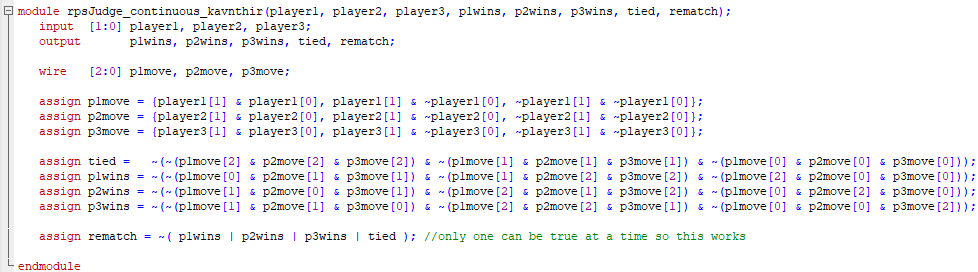
\includegraphics[width = .98\textwidth]{code.png}}
\end{center}
\section{RPS Continuous Test Bench}
\begin{center}
    \boxed{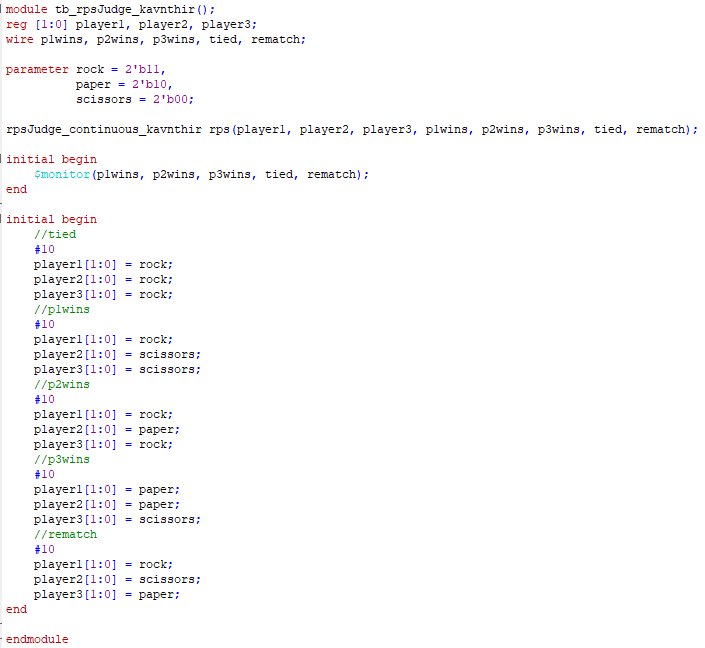
\includegraphics[width = .98\textwidth]{tb.png}}
\end{center}

The simulation approach I did this time was to test out specific cases for each output to see if the proper result was achieved, and for the cases I ran the output was correct. Because circuits like this are very particular, in the way where if one thing is wrong everything is wrong, this is a good way to test because its easy to understand and visualize. I also changed the inputs on the test bench for different cases to test if they also worked. Output for simulation can be seen in below section for reference.

\subsection{RPS Simulation}

\begin{center}
    \boxed{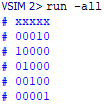
\includegraphics[width = .20\textwidth]{sim.png}}
\end{center}


\section{Conclusion}

I learned in this assignment that by taking the time to think about the problem a little bit more a complicated mess of truth tables and kmaps can be turned into a simple easy to implement problem. So by approaching every digital circuit like this it would become much easy to not only design but when the time comes to debug these circuits.

\end{document}
